\graphicspath{{Kapitel/Kapitel3_Grundlagen/Images/}}

Dieses Kapitel befasst sich mit einigen grundlegenden Themen, die mit dem Inhalt dieser Arbeit zu tun haben. Dies soll dem besseren Verständnis für die folgenden Kapitel dienen. Der Abschnitt \ref{sec:MLearning} beispielsweise, befasst sich mit dem Prinzip des maschinellen Lernens auf Basis von neuronalen Netzen, was verdeutlichen soll warum die Daten der Punktwolken überhaupt \glslink{glos:Labeling}{gelabelt} werden müssen. Anschließend wird die CMORE Inhouse Software C.LABEL in \ref{sec:C.LABEL} vorgestellt um den aktuellen Stand der Technik im Bereich Punktwolkenannotierung zu zeigen. \ref{sec:UnityEngine} stellt die \glslink{glos:GameEngine} Unity vor, die benutzt wurde um die \acrlong{acr:VR} Applikation zu erstellen.

\section{Maschinelles Lernen}
\label{sec:MLearning}
Der Ausdruck Maschinelles Lernen (engl.: \textit{Machine Learning}) ist heutzutage ein Überbegriff für Methoden, die versuchen durch Optimierung eine Funktion zu erlernen. Bei solch einer Funktion kann es sich sowohl um eine simple binäre Entscheidung auf eine Fragestellung handeln als auch um komplexere Dinge wie das Übersetzen von Texten in eine andere Sprache, das Erkennen von Personen auf Bildern, oder eben das Klassifizieren von Objekten in einer Punktwolke, was für diese Arbeit relevant ist. Die Komplexität der Funktion bestimmt auch die zu verwendende Methode zur Lösung des Problems. Im Zuge des Azure Machine Learning Studios veröffentlichte Microsoft eine Graphik (vgl. Abbildung \ref{fig:MLCS}), mit der man den richtigen Lernalgorithmus für gewisse \glslink{glos:PredAna}{Predictive-Analytics-Methoden} bestimmen kann. Für die Objektklassifizierung im Automobilbereich ist es wichtig die Klasse eines Objekts mit hoher Genauigkeit aus einer großen Anzahl verschiedener Klassen zu bestimmen. Basierend auf der Graphik \ref{fig:MLCS} ist die beste Methode dafür ein Künstliches Neuronales Netz(\acrshort{acr:knn}). Die Benutzung solcher Netze ist üblich, wenn es um Klassifikation von vielen verschiedenen Dingen geht und soll im folgenden näher erläutert werden.

\begin{figure}%
	\centering
    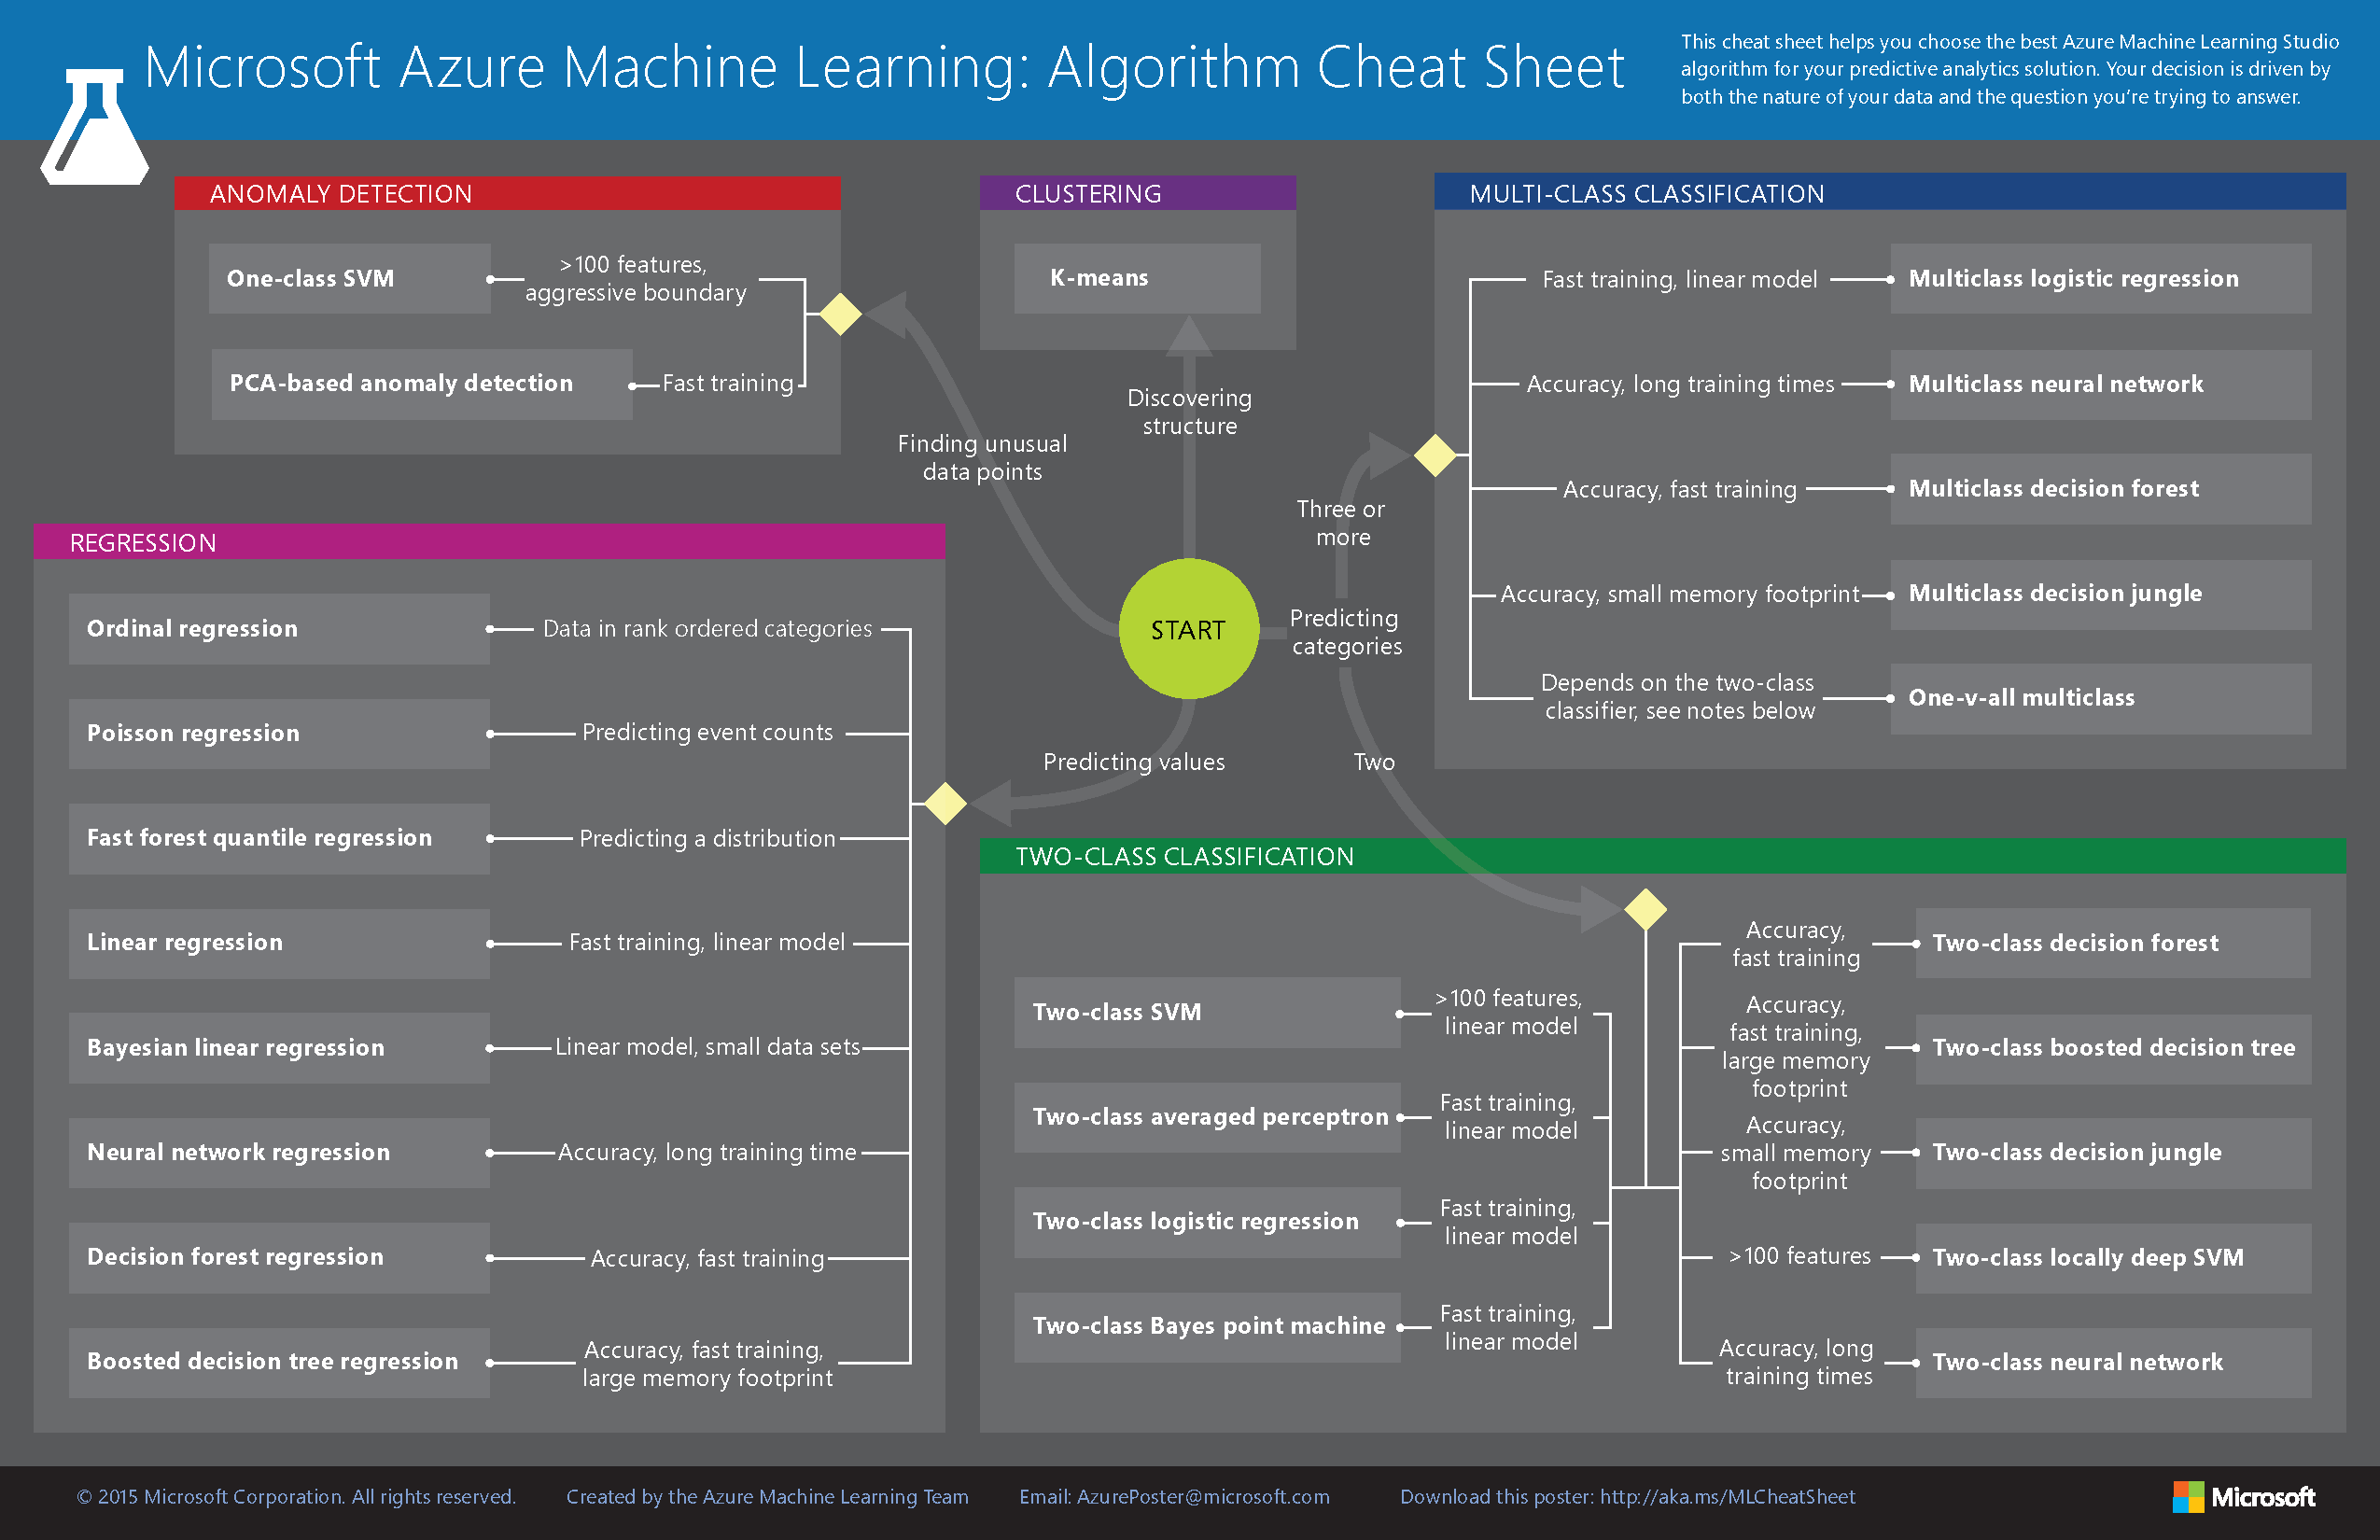
\includegraphics[width=19cm, angle=270]{MLCS}
    \caption{Diagramm um den besten Machine Learning Algorithmus für eine \glslink{glos:PredAna}{Predictive-Analytics-Methoden} zu finden}
    \label{fig:MLCS}
\end{figure}
  
\subsection{Künstliche Neuronale Netze}
Das Prinzip der Künstlichen Neuronalen Netze ist, wie vieles in der Informatik, einer Struktur aus der realen Welt nachempfunden. Das komplexeste neuronale Netz ist wohl das menschliche Gehirn mit etwa 86 Milliarden Nervenzellen, welche auch Neuronen genannt werden. Daher kommt auch der Begriff des Neuronalen Netzes. Diese Nervenzellen sind durch Synapsen mit bis zu mehreren Tausend anderen Zellen verbunden. Diese Verbindungen bilden zusammen das Netz. Die Kommunikation zwischen den Neuronen erfolgt in der Regel über elektrische Impulse oder chemische Botenstoffe. Beides wird über Synapsen zu den nächsten, verbundenen Neuronen weitergeleitet und bewirkt dort einen Reiz. Bei der Übertragung von chemischen Botenstoffen kann dieser Reiz zusätzlich gewichtet werden, das heißt es kann ein stärkerer oder schwächerer Reiz ausgesendet werden. Alle ankommenden Reize werden dann am Empfangsneuron akkumuliert und ergeben den Eingangsreiz des Neurons. Dieses, vereinfacht dargestellte Prinzip, wird auch bei den  \acrshort{acr:knn}s verwendet. Übersteigt dieser Reiz eine bestimmte Schwelle kommt es zum entscheidenden Ereignis: Das Neuron \textit{feuert}. Dadurch gibt das feuernde Neurone einen Impuls an alle anderen Neuronen weiter mit dem es verbunden ist. Bei dafür vorgesehenen Neuronen oder verbänden davon, kann dieser Impuls auch ein Ereignis auslösen. Diese Ereignisse können physischer Natur sein, also beispielsweise Bewegungen, oder auch psychischer Natur, zum Beispiel das Erkennen von Dingen. Werden diese Nervenzellen mit einem Ausreichenden Impuls angesprochen, wird das entsprechende Ereignis ausgelöst.\\

Die entscheidende Komponente dieses Prinzips ist die adaptive Gewichtung der weitergegebenen Reize. Adaptiv deswegen, da die Gewichtung der Reize sich während eines Menschenlebens verändern können. So erkennen Kinder oft Gefahrensituation nicht, da ihr Gehirn nicht ausreichend geschult ist um diese zu erkennen. In diesem Kontext bedeutet das, dass an die {\glqq Gefahren-Neuronen\grqq} kein ausreichend starker Reiz gesendet wird. Durch sammeln von Erfahrungen optimiert sich dieser Wert, was in späteren Jahren zu einer anderen Reaktion des Gehirns führen kann als früher. Das adaptieren dieser Gewichte auf einen passenden Wert bezeichnen wir als Lernen. Um Computersystemen einen derartigen Lerneffekt zu ermöglichen wurde dieses Biologische Prinzip nun mathematisch imitiert. \\

\begin{figure}%
	\centering
    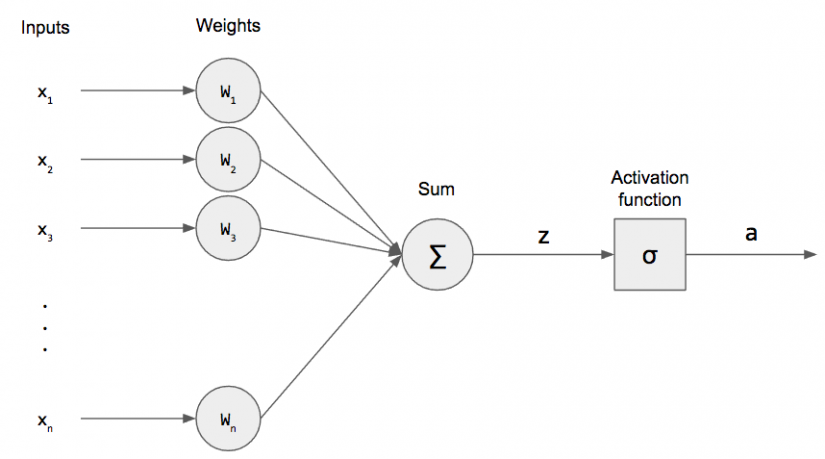
\includegraphics[width=13cm]{Perceptron}
    \caption{Einfaches Perzeptron nach dem Prinzip von Frank Rosenblatt}
    \label{fig:Perceptron}
\end{figure}

Künstliche Neuronale Netze basieren auf dem Prinzip des Perzeptrons, das von Frank Rosenblatt 1958 vorgestellt wurde \cite{bib:Perzeptron}. Dieses Perzeptron repräsentiert die Funktion eines Neuron auf eine mathematische Weise (vgl. \ref{fig:Perceptron}). Die Eingangsdaten eines Perzeptrons bestehen aus einer \(n\)-großen Menge an Werten \(x_1 \dots x_n\), welche eine gleichgroße Menge an jeweiligen Gewichten \(W_1 \dots W_n\) haben. Wenn das zu analysierende Ziel beispielsweise ein Bild ist, wäre \(n\) die Menge aller Pixel des Bildes und bei Punktwolken eben die Anzahl der Punkte. Die Eingangswerte werden von einer mathematischen Funktion empfangen und zu einem skalaren Wert \(z\) zusammengefasst. Hierbei wird meist die Gewichtete Summe benutzt die folgendermaßen berechnet wird:

\begin{equation}
z = \sum \limits_{i=0}^{n} W_i \cdot x_i
\end{equation}\\

Im biologischen Vorbild repräsentiert diese Summe den eingehenden Reiz in eine Nervenzelle, die \(x\)-Werte sind dabei die Impulse der vorherigen Neuronen und die \(W\)-Werte repräsentieren die Gewichtung, also die Stärke der Eingangsreize. Der biologische Schwellwert wird im Perzeptron durch eine Mathematische Funktion \(\sigma(z)\) dargestellt. Wie in \cite{bib:NeuronaleNetze} beschrieben gibt dafür es zwei beliebte Funktionen. Die \textit{Fermifunktion} (\ref{eq:Fermi}) , auch Logische Funktion genannt, welche einen Ausgabe-Wertebereich von (0,1) hat und den \textit{Tangens Hyperbolicus} (\(tanh(z)\)) mit einem Wertebereich von (-1,1). Beide sind differenzierbar, was wichtig für das Lernen mit Backpropagation ist. Was das bedeutet wird in \ref{sec:Training} näher erläutert. Wenn der Wert, den diese Funktion liefert, nicht noch durch eine weitere Ausgangsfunktion verändert wird, ist er der Ausgangswert des Perzeptrons.

\begin{equation}
\sigma(z) = \frac{1}{1 + e^-z}
\label{eq:Fermi}
\end{equation}

In \acrshort{acr:knn}s können mehrere dieser Perzeptrons eine sogenannte Schicht bilden. Je mehr Schichten ein neuronales Netz hat desto \textit{tiefer} ist es, daher auch der Begriff \textit{Deep Learning}, also tiefes Lernen. In der Regel bestehen \acrshort{acr:knn}s aus mindestens 3 Schichten, nämlich einer Eingangsschicht, einer oder mehrerer Zwischenschichten und einer Ausgangsschicht.

\subsubsection{Eingangschicht}
Die Eingabeschicht ist der Startpunkt des Informationsflusses in einem künstlichen neuronalen Netz. Eingangssignale werden von den Neuronen dieser Schicht aufgenommen und gewichtet an alle Neuronen der ersten Zwischenschicht weitergegeben. Die Anzahl der Neuronen dieser Schicht hängt, wie schon erwähnt, von den Eingangsdaten ab. Werden Bilder mit einer Auflösung von 50x50 in das Netz gespeist, hat dieses Netz in der Regel 50x50, also 2500 Neuronen in der Eingangsschicht.

\subsubsection{Zwischenschicht}
Zwischen der Eingabe- und der Ausgabeschicht befindet sich in jedem künstlichen neuronalen Netz mindestens eine Zwischenschicht, die auch verborgene Schicht(engl.: \textit{hidden layer}) genannt wird. Theoretisch ist die Anzahl der möglichen verborgenen Schichten in einem künstlichen neuronalen Netzwerk unbegrenzt. In der Praxis bewirkt jede hinzukommende Schicht jedoch auch einen Anstieg der benötigten Rechenleistung, die für den Betrieb des Netzes notwendig ist.

\subsubsection{Ausgangsschicht}
Die Ausgabeschicht liegt hinter den Zwischenschichten und bildet die letzte Schicht in einem Künstlichen Neuronalen Netz. In der Ausgabeschicht angeordnete Neuronen sind jeweils mit allen Neuronen der letzten Zwischenschicht verbunden. Die Ausgabeschicht stellt den Endpunkt des Informationsflusses in einem \acrshort{acr:knn} dar und enthält das Ergebnis der Informationsverarbeitung durch das Netzwerk. Beim Beispiel der Objektklassifikation besteht die Ausgabeschicht nun aus \(n\) vielen Endknoten, wobei \(n\) die Menge an möglichen Klassifikationen ist. Die Eingangssumme dieser Knoten, den sie aus den vorherigen Neuronen bekommen, entsprechen der Wahrscheinlichkeit, dass es sich bei den Eingangsdaten um die jeweilige Klasse handelt. Abbildung \ref{fig:Bilderkennung} soll dieses Prinzip nochmals veranschaulichen. 

\begin{figure}%
	\centering
    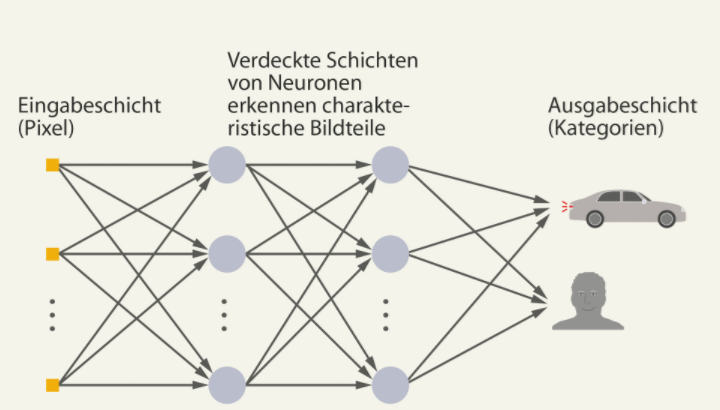
\includegraphics[width=13cm]{Bilderkennung}
    \caption{Stark vereinfachte Darstellung eines \acrshort{acr:knn}s zur Erkennung von Autos und Personen}
    \label{fig:Bilderkennung}
\end{figure}

\subsection{Trainieren von Neuronalen Netzen}
\label{sec:Training}

Lernen ist ein weiter Begriff. Es bedeutet, dass ein System sich in irgendeiner Form verändert, um sich z.B. an Veränderungen in seiner Umwelt anzupassen. Die typische Veränderung von künstlichen neuronalen Netzen ist das adaptieren der Verbindungsgewichte \(W_1 \dots W_n\). Diese Adaption geschieht nach Regeln, die man in Algorithmen definiert – ein Lernverfahren ist also immer ein Algorithmus, den man einfach mithilfe einer Programmiersprache implementieren kann. Diese Algorithmen lassen sich grob in 3 verschieden Arten einteilen, nämlich Unüberwachtes Lernen (\textit{Unsupervised Learning}), Bestärkendes Lernen (\textit{Reinforcement Learning}) und Überwachtes Lernen (Supervised Learning). Für Objektklassifizierung wird in der Regel letzteres verwendet, darum wird im Folgenden nur auf das Supervised Learning eingegangen.\\
 
Der Lernprozess bei dieser Methode ist, wie der Name schon sagt, überwacht. Das kommt daher, dass das Netz von einer, vom Menschen vordefinierten, Menge an Trainingsbeispielen lernt. Genauer gesagt sind diese Beispiele eine Menge \(P\) an Eingabemustern mit jeweiliger korrekter Lösung, sodass das Netz nach der Ausgabe eine gewisse Fehlerbeschreibung zurückgeben kann. Für das Beispiel der Punktwolkenklassifizierung bestünde dabei das Trainingsset aus vielen verschiedenen Punktwolken, die alle ein Objekt darstellen, wobei die Art des Objektes, also die Lösung der Klassifizierung, bekannt ist. \\

Die Werte der Gewichte \(W_1 \dots W_n\) werden bei einem untrainierten Netz zu Beginn zufällig gewählt. Dadurch gibt ein solches Netz in der Regel völlig falsche Lösungen für die ersten Trainingsbeispiele aus. Das ist aber nicht weiter schlimm, da nun der Lerneffekt einsetzen soll. Durch die Bekanntheit der Lösung des Beispiels kann der Fehler zwischen dem Ergebnis des Netzes und der gewünschten Lösung genau bestimmt werden. Dieser Fehler kann durch zurückrechnen auf jedes Neuron projiziert werden und so kann der Fehler, den jedes einzelne Neuron verursacht bestimmt werden. Daraus kann dann der Betrag errechnet werden, um den sich das Gewicht \(W_i\) des Neurons verändern muss, damit bei zukünftigen Eingaben bessere Ergebnisse erzielt werden. Dieses Zurückrechnen nennt sich \textit{Backpropagation}. Für das Verständnis des Grundprinzips ist die Formel zu Berechnung der Gewichtsänderung nicht wichtig, sie wird aber zur Vervollständigung im Folgenden angegeben: 

\begin{equation}
\triangle w_{ij} = -\eta\delta_jo_i
\label{eq:BackProb}
\end{equation}

\begin{itemize}
\item \(\triangle w_{ij}\) ist die Änderung des Gewichts \(w_{ij}\) der Verbindung von Neuron \(i\) zu Neuron \(j\)
\item \(\eta\)  ist ein fester Wert, der eine Lernrate ausdrücken soll, mit der die Stärke der Gewichtsveränderung festgelegt wird
\item \(\delta_j\) ist das Fehlersignal des Neurons \(j\) das sich aus der partiellen Ableitung \(\frac{\partial E}{\partial net_j}\) ergibt\\
\begin{itemize}
\item \(E\) ist dabei der quadratische Fehler der bei der Berechnung des Ergebnisses entstand, er wird durch die Formel \(E = \sum \limits_{i=1}^n (t_i - o_i)^2\) berechnet
\begin{itemize}
\item \(t_i\) steht darin für den gewünschten Zielwert
\end{itemize}
\item \(net_j\) ist die Netzeingabe \(\sum \limits_{i=1}^n x_iw_{ij}\)
\end{itemize}

\item \(o_i\) steht sowohl bei der Berechnung von \(\triangle w_{ij}\), als auch von \(E\) für die errechnete Ausgabe des Neurons \(i\)
\end{itemize}

Zusammenfassend kann man nun sagen, dass der Lernprozess eines künstlichen Neuronalen Netzes nach folgendem Schema abläuft:

\begin{enumerate}
\item \textbf{Eingabe} eines Elements \(p\) aus der Trainingsmenge \(P\) in die Eingabeschicht des Netzes
\item \textbf{Vorwärtspropagierung} der Eingabe durch das Netz gesamte Netz, sodass man bei der Ausgabeschicht ein Ergebnis erhält
\item \textbf{Vergleich} des Ergebnisses mit der richtigen Lösung und Berechnung des Fehlers
\item \textbf{Zurückpropagieren} des Fehlers, um somit die Gewichte der Neuronen anzupassen
\end{enumerate}

Wie unschwer zu erkennen ist basiert der Backpropagation-Algorithmus auf dem Vorhandensein eines Trainingsdatensatzes. Damit das Netz nach dem Training für neue, unbekannte Eingaben die richtige Lösung errechnet ist es elementar wichtig, dass dieser Datensatz eine hohe Qualität und Quantität hat. Qualität bedeutet in diesem Fall, dass die Trainingsdaten repräsentativ für den jeweiligen Anwendungsfall sein müssen. Ein Personenerkennungsalgorithmus der im Straßenverkehr Personen identifizieren soll liefert keine guten Ergebnisse, wenn er ausschließlich mit Bildern von Personen in Innenräumen gefüttert wird. Mit Quantität ist Anzahl der verschiedenen Elemente im Trainingssatz gemeint. \acrshort{acr:knn}s verbessern ihre Ausgabe in der Regel mit größerer Menge an unterschiedlichen Trainingsdaten.\\

Zur Erstellung dieses Datensatzes ist es nun nötig so viele repräsentative Daten wie möglich zu sammeln und diese mit der richtigen Lösung zu annotieren. Eine Methode für eine solche Annotierung wird in dieser Arbeit vorgestellt. Dieses Kapitel sollte nun veranschaulicht haben warum  solche Methoden so essentiell, auf dem Weg zur Erschaffung einer künstlichen Intelligenz, sind.

\section{Das C.LABEL Tool}
\label{sec:C.LABEL}
%TODO 
Beschreibung des C.Label Tools, was es kann, was in die VR übernommen werden soll und was deswegen für die weitere Auswahl an HW und Tools zu berücksichtigen ist

\section{Die Unity Engine}
\label{sec:UnityEngine}

